\documentclass[conference,a4paper]{IEEEtran}
\IEEEoverridecommandlockouts
\usepackage{cite}
\usepackage{amsmath,amssymb}
\usepackage{graphicx}
\usepackage{booktabs}
\usepackage{multirow}
\usepackage{array}
\newcolumntype{L}[1]{>{\raggedright\arraybackslash}p{#1}}
\usepackage{algorithm}
\usepackage{algpseudocode}
\usepackage{tikz}
\usetikzlibrary{arrows.meta,positioning,fit,calc}
\usepackage[hidelinks]{hyperref}
\usepackage{xcolor}

\begin{document}

\title{Vectorised Execution versus Multi-Core Parallelism: Benchmarking Pandas, Polars and DuckDB on Group-By and Join Queries}

\author{
\IEEEauthorblockN{Krish}
\IEEEauthorblockA{Roll No. 25124053\\
Dept. of Information Technology\\
Dr B R Ambedkar NIT Jalandhar\\
krish2.it.25@nitj.ac.in}
\and
\IEEEauthorblockN{Krish Singhal}
\IEEEauthorblockA{Roll No. 25124054\\
Dept. of Information Technology\\
Dr B R Ambedkar NIT Jalandhar\\
krishs.it.25@nitj.ac.in}
\and
\IEEEauthorblockN{Laksh Kapoor}
\IEEEauthorblockA{Roll No. 25124055\\
Dept. of Information Technology\\
Dr B R Ambedkar NIT Jalandhar\\
lakshk.it.25@nitj.ac.in}
\and
\IEEEauthorblockN{Lucky}
\IEEEauthorblockA{Roll No. 25124056\\
Dept. of Information Technology\\
Dr B R Ambedkar NIT Jalandhar\\
lucky.it.25@nitj.ac.in}
}

\maketitle

\begin{abstract}
Analytical queries such as group-by aggregation and joins dominate data-science workloads, yet the most widely used Python tool for them, Pandas, was not designed around modern CPU features. Vectorised engines such as DuckDB and Polars process data column by column in cache-sized batches that suit SIMD instructions and multi-core CPUs, and GPU engines push the same idea further. Reported speed-ups, however, rarely separate the gain that comes from the execution model itself from the gain that comes from extra cores. We review 18 studies on vectorised, SIMD, GPU and columnar query processing, and benchmark Pandas, Polars and DuckDB on a group-by query and a join-plus-aggregate query over synthetic tables of 1, 5 and 10 million rows. To separate the two effects, DuckDB is run on one thread and on all available threads. All engines return identical results. At 10 million rows, single-threaded DuckDB is 3.4$\times$ (group-by) and 5.6$\times$ (join) faster than Pandas; the second core adds a further 1.4--1.8$\times$, giving 6.2$\times$ and 7.7$\times$ overall, while Polars is 5.1$\times$ and 5.9$\times$ faster. Gains grow with data size and are largest for the join, where Pandas materialises the whole joined table. We conclude that on commodity hardware most of the benefit comes from vectorised columnar execution rather than from parallelism. All code and data generators are publicly available.
\end{abstract}

\begin{IEEEkeywords}
vectorised execution, query processing, SIMD, columnar storage, Apache Arrow, GPU database
\end{IEEEkeywords}

%======================================================================
\section{Introduction}
Consider a data analyst at an online retailer who must summarise ten million orders by store and by customer segment several times a day while exploring the data in a notebook. In Pandas, the de-facto Python dataframe library~\cite{mckinney10}, a join followed by an aggregation over such a table takes well over a second on a laptop; repeated across hundreds of interactive steps, that delay shapes how the analyst works. Newer engines promise far better performance on the same hardware. DuckDB is an in-process analytical database~\cite{raasveldt19}, and Polars is an Arrow-based dataframe library~\cite{polars,arrow}. Behind them lies two decades of research on making query processing fit modern processors: vectorised execution~\cite{boncz05}, SIMD-aware operators~\cite{polychroniou15}, columnar formats~\cite{zeng23} and GPU acceleration~\cite{shanbhag20,paul21}.

\textbf{Problem statement.} Speed-up figures for these engines are easy to find, but they mix two different causes: a better \emph{execution model} (columnar, vectorised, SIMD-friendly code) and \emph{more hardware} (multiple cores, or a GPU). For a student, a data scientist or a system designer, the distinction matters: the first gain is available on any machine, the second only on machines with many cores or an accelerator. This paper asks how large each part is for two of the most common analytical operations.

We answer three research questions:
\begin{itemize}
\item \textbf{RQ1:} How do vectorised and GPU engines execute queries, and how does this differ from Pandas?
\item \textbf{RQ2:} What role do SIMD, columnar formats and Apache Arrow play in their performance?
\item \textbf{RQ3:} What speed-up do they achieve on group-by and join queries, and how much of it comes from the execution model rather than from extra cores?
\end{itemize}

\textbf{Contributions.} (1)~A thematic review of 18 studies on vectorised, GPU and columnar query processing, with a comparison table and an explicit research gap. (2)~A small, fully reproducible benchmark of Pandas, Polars and DuckDB on group-by and join queries at three data sizes, with automatic result-equality checks. (3)~A simple decomposition of DuckDB's speed-up into an execution-model factor (one thread) and a parallelism factor (all threads). (4)~An explanation of why the gains arise, linked to the literature.

The rest of the paper is organised as follows. Section~\ref{sec:background} gives background. Section~\ref{sec:related} reviews related work. Section~\ref{sec:method} describes our approach and Section~\ref{sec:setup} the experimental setup. Section~\ref{sec:results} answers RQ1--RQ3, and Section~\ref{sec:conclusion} concludes.

%======================================================================
\section{Background}\label{sec:background}
\textbf{Tuple-at-a-time execution.} Classic database engines follow the Volcano iterator model~\cite{graefe94}: every operator calls \texttt{next()} on its child to obtain one row at a time. This is simple and composable, but it spends most CPU cycles on function calls and interpretation rather than on the actual arithmetic, and it prevents the compiler from using SIMD instructions~\cite{boncz05}.

\textbf{Vectorised execution.} MonetDB/X100~\cite{boncz05} keeps the iterator structure but passes a \emph{vector} of values from one column (in DuckDB, 2048 values) between operators instead of a single row (Fig.~\ref{fig:model}). Each operator then runs a tight loop over a small array that fits in the CPU cache. The interpretation overhead is paid once per vector instead of once per row, and the loops can use SIMD (Single Instruction, Multiple Data) instructions such as AVX2, which apply one operation to 4--16 values at once~\cite{polychroniou15}. An alternative, data-centric code generation, compiles a whole pipeline into machine code; both approaches are competitive~\cite{kersten18}.

\textbf{Columnar layout and Apache Arrow.} Vectorised operators work best when the values of one column are stored contiguously. Columnar file formats such as Parquet store data this way on disk~\cite{zeng23}, and Apache Arrow defines a standard columnar layout in memory~\cite{arrow}, so that engines such as Polars and DataFusion~\cite{lamb24} can process data without converting it.

\textbf{Parallelism and accelerators.} On top of the execution model, engines split the input into chunks processed by several CPU threads. GPUs extend this to thousands of threads and much higher memory bandwidth, at the cost of moving data to the GPU~\cite{shanbhag20,rosenfeld23}.

\begin{figure}[t]
\centering
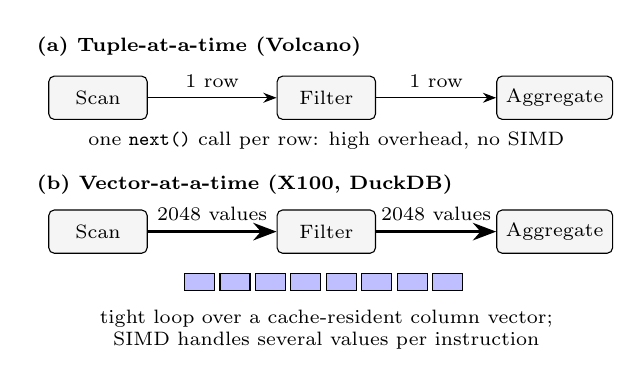
\begin{tikzpicture}[
  op/.style={draw, rounded corners=2pt, minimum width=1.25cm, minimum height=0.55cm, font=\scriptsize, fill=gray!8},
  lab/.style={font=\scriptsize\bfseries, anchor=west},
  note/.style={font=\scriptsize, align=center},
  >=Stealth]
\node[lab] at (-0.2,1.15) {(a) Tuple-at-a-time (Volcano)};
\node[op] (s1) at (0.7,0.5) {Scan};
\node[op] (f1) at (3.6,0.5) {Filter};
\node[op] (a1) at (6.5,0.5) {Aggregate};
\draw[->] (s1) -- node[note, above]{1 row} (f1);
\draw[->] (f1) -- node[note, above]{1 row} (a1);
\node[note] at (3.6,-0.05) {one \texttt{next()} call per row: high overhead, no SIMD};
\node[lab] at (-0.2,-0.6) {(b) Vector-at-a-time (X100, DuckDB)};
\node[op] (s2) at (0.7,-1.2) {Scan};
\node[op] (f2) at (3.6,-1.2) {Filter};
\node[op] (a2) at (6.5,-1.2) {Aggregate};
\draw[->, very thick] (s2) -- node[note, above]{2048 values} (f2);
\draw[->, very thick] (f2) -- node[note, above]{2048 values} (a2);
\foreach \i in {0,...,7} { \draw[fill=blue!25] (1.8+\i*0.45,-1.95) rectangle ++(0.38,0.22); }
\node[note, text width=7cm] at (3.6,-2.45) {tight loop over a cache-resident column vector;\\ SIMD handles several values per instruction};
\end{tikzpicture}
\caption{Tuple-at-a-time versus vectorised query execution.}
\label{fig:model}
\end{figure}

%======================================================================
\section{Related Work}\label{sec:related}
We searched Google Scholar, ACM DL, IEEE Xplore and arXiv with the keywords \emph{vectorised execution}, \emph{GPU database} and \emph{Apache Arrow}, starting from the DuckDB paper~\cite{raasveldt19}. Of the 18 studies selected, 13 (72\%) were published in 2021 or later. We group them into three themes.

\subsection{Vectorised CPU Execution and SIMD}
Boncz et al.~\cite{boncz05} found that row-at-a-time engines leave a modern CPU mostly idle during analytical queries. Their MonetDB/X100 prototype, which pipelines small column vectors instead, ran TPC-H between 10 and 100 times faster than earlier systems. Polychroniou et al.~\cite{polychroniou15} rebuilt the core database operators, from scans and hash tables to sorts and joins, around advanced SIMD instructions that read and write scattered memory locations, and report gains of up to ten times over scalar code. Kersten et al.~\cite{kersten18} built both a vectorised and a compiled engine inside one test system and found that neither always wins: the vectorised design copes better with memory stalls, whereas the compiled design needs fewer CPU instructions. The model is now standard in industry. DuckDB brings it to an embedded library~\cite{raasveldt19}. Photon re-implements Spark execution as a native vectorised engine, with an average 3$\times$ speed-up for customers~\cite{behm22}, and Meta's Velox packages vectorised operators as a reusable library~\cite{pedreira22}. Recent DuckDB work keeps group-by and join fast when intermediates exceed memory~\cite{kuiper24,kuiper25}.

\subsection{GPU and New Hardware}
GPU databases claim speed-ups of 2$\times$ to 100$\times$, but Shanbhag et al.~\cite{shanbhag20} show that many of these figures come from weak CPU baselines; against optimised CPU code, the GPU advantage (25$\times$ on the Star Schema Benchmark) is explained largely by memory bandwidth. Surveys by Paul et al.~\cite{paul21} and Rosenfeld et al.~\cite{rosenfeld23} describe GPU-specific data layouts and operators, and the main obstacle: moving data over the PCIe bus. Mordred~\cite{yogatama22} reduces this by caching hot data on the GPU and co-executing queries on the CPU and GPU. Cao et al.~\cite{cao23} find that GPU databases often leave the GPU under-used. Beyond GPUs, Daase et al.~\cite{daase21} show that persistent memory (Intel Optane) runs read-heavy analytical queries only 1.66$\times$ slower than DRAM, a cheaper way to hold large data in memory.

\subsection{Columnar Formats, Arrow and Dataframes}
Zeng et al.~\cite{zeng23} and Liu et al.~\cite{liu23} evaluate Parquet, ORC and Arrow, and recommend designs that favour fast decoding and vectorised processing. DataFusion~\cite{lamb24} shows that an engine built directly on Arrow can be both modular and fast. Closest to our work, Mozzillo et al.~\cite{mozzillo25} compare Pandas with Polars, cuDF, Modin and others for data preparation, and recommend Polars when data fits in RAM and cuDF when a GPU is available.

\subsection{Comparison and Research Gap}
Table~\ref{tab:compare} compares nine key papers. Two patterns stand out. First, most evaluations use data-centre CPUs or GPUs, full DBMSs, or proprietary systems that students cannot reproduce. Second, studies that compare tools end to end~\cite{mozzillo25} report \emph{how much} faster an engine is, but not \emph{why}: they do not separate the gain from the execution model from the gain from extra cores. \textbf{Gap:} there is little reproducible, commodity-hardware evidence on how much of an embedded engine's speed-up over Pandas comes from vectorised execution alone. We address this by running DuckDB with one thread and with all threads.

\begin{table*}[t]
\centering
\caption{Comparison of key related work}
\label{tab:compare}
\footnotesize
\setlength{\tabcolsep}{4pt}
\begin{tabular}{@{}L{2.7cm}L{1.9cm}L{2.2cm}L{3.0cm}L{2.3cm}L{4.4cm}@{}}
\toprule
\textbf{Work} & \textbf{Venue} & \textbf{Hardware} & \textbf{Approach} & \textbf{Workload} & \textbf{Key finding} \\
\midrule
Boncz et al.~\cite{boncz05} & CIDR 2005 & CPU & Vectorised engine (X100) & TPC-H 100 GB & 10--100$\times$ over earlier engines \\
Polychroniou et al.~\cite{polychroniou15} & SIGMOD 2015 & CPU, Xeon Phi & SIMD operator designs & Micro-benchmarks & Up to 10$\times$ over scalar code \\
Kersten et al.~\cite{kersten18} & PVLDB 2018 & Multi-core CPU & Vectorised vs compiled & TPC-H subset & Both fast; different strengths \\
Raasveldt \& M\"uhleisen~\cite{raasveldt19} & SIGMOD 2019 & CPU & Embedded vectorised DBMS & Demo & In-process OLAP is practical \\
Shanbhag et al.~\cite{shanbhag20} & SIGMOD 2020 & GPU vs CPU & Crystal GPU library & SSB & 25$\times$, mostly memory bandwidth \\
Daase et al.~\cite{daase21} & SIGMOD 2021 & Persistent memory & PMem for OLAP & SSB & 1.66$\times$ slower than DRAM \\
Behm et al.~\cite{behm22} & SIGMOD 2022 & Cloud cluster & Native vectorised engine & TPC-DS, customers & 3$\times$ average over previous engine \\
Cao et al.~\cite{cao23} & PVLDB 2023 & Data-centre GPU & GPU DBMS characterisation & Analytical queries & GPUs often under-used \\
Mozzillo et al.~\cite{mozzillo25} & EDBT 2025 & CPU, GPU & Dataframe library comparison & Real data, TPC-H & Polars best in RAM; cuDF with GPU \\
\midrule
\textbf{This work} & -- & 2-core commodity CPU & 1-thread vs all-thread split & Synthetic, 1--10M rows & 3.4--5.6$\times$ from execution model alone \\
\bottomrule
\end{tabular}
\end{table*}

%======================================================================
\section{Proposed Approach}\label{sec:method}
Fig.~\ref{fig:arch} shows our benchmark pipeline. A generator creates two tables with a fixed random seed and stores them as Parquet files. Each engine loads the tables into its own in-memory format before timing starts, so only query execution is measured. A harness then runs every query on every engine, checks that all engines return the same answer, and writes the timings to a CSV file from which all figures are drawn.

\begin{figure}[t]
\centering
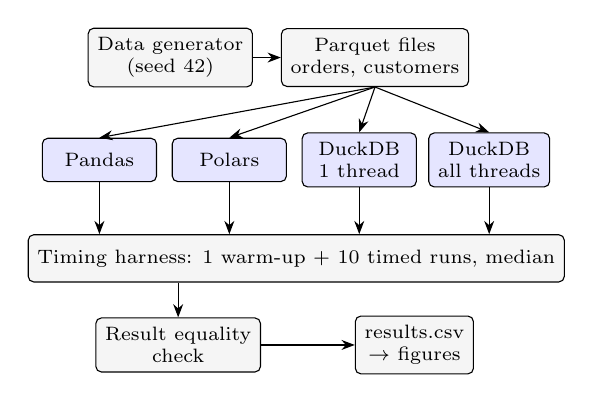
\begin{tikzpicture}[
  box/.style={draw, rounded corners=2pt, align=center, font=\scriptsize, minimum height=0.6cm, fill=gray!8},
  eng/.style={draw, rounded corners=2pt, align=center, font=\scriptsize, minimum width=1.45cm, minimum height=0.55cm, fill=blue!10},
  >=Stealth]
\node[box] (gen) at (0,0) {Data generator\\(seed 42)};
\node[box] (pq) at (2.6,0) {Parquet files\\orders, customers};
\node[eng] (e1) at (-0.9,-1.3) {Pandas};
\node[eng] (e2) at (0.75,-1.3) {Polars};
\node[eng] (e3) at (2.4,-1.3) {DuckDB\\1 thread};
\node[eng] (e4) at (4.05,-1.3) {DuckDB\\all threads};
\node[box, minimum width=6.3cm] (h) at (1.6,-2.55) {Timing harness: 1 warm-up + 10 timed runs, median};
\node[box] (chk) at (0.1,-3.65) {Result equality\\check};
\node[box] (out) at (3.1,-3.65) {results.csv\\$\rightarrow$ figures};
\draw[->] (gen) -- (pq);
\foreach \e in {e1,e2,e3,e4} { \draw[->] (pq.south) -- (\e.north); \draw[->] (\e.south) -- (\e.south |- h.north); }
\draw[->] (h.south -| chk) -- (chk);
\draw[->] (chk) -- (out);
\end{tikzpicture}
\caption{Architecture of the benchmark pipeline.}
\label{fig:arch}
\end{figure}

\textbf{Workload.} The \texttt{orders} table has $N$ rows (order id, customer id, store id, quantity, amount), and the \texttt{customers} table has $N/10$ rows (customer id, segment, credit limit). This one-to-ten ratio mimics the fact-to-dimension join of a star schema. We run two queries:

\smallskip\noindent\textbf{Q1 (group-by, 100 groups):}\\
{\footnotesize\ttfamily\raggedright SELECT store\_id, SUM(amount),\\ \hspace*{1em}AVG(quantity), COUNT(*)\\ \hspace*{1em}FROM orders GROUP BY store\_id\par}

\smallskip\noindent\textbf{Q2 (join + group-by, 5 groups):}\\
{\footnotesize\ttfamily\raggedright SELECT c.segment, SUM(o.amount), COUNT(*)\\ \hspace*{1em}FROM orders o JOIN customers c\\ \hspace*{1em}ON o.customer\_id = c.customer\_id\\ \hspace*{1em}GROUP BY c.segment\par}
\smallskip

DuckDB runs the SQL directly. The same logic is written idiomatically in Pandas (\texttt{groupby}, \texttt{merge}) and in Polars (lazy \texttt{group\_by}, \texttt{join}).

\begin{algorithm}[t]
\caption{Benchmark harness}
\label{alg:harness}
\begin{algorithmic}[1]
\Require sizes $\mathcal{N}$, engines $\mathcal{E}$, queries $\mathcal{Q}$, runs $R{=}10$
\For{$N \in \mathcal{N}$}
  \State generate \texttt{orders}($N$), \texttt{customers}($N/10$); write Parquet
  \State load both tables into memory for every $e \in \mathcal{E}$
  \For{$e \in \mathcal{E}$, $q \in \mathcal{Q}$}
    \State run $q$ on $e$ once \Comment{warm-up, not timed}
    \For{$r = 1$ \textbf{to} $R$}
      \State $t_r \gets$ wall-clock time of $q$ on $e$
    \EndFor
    \State record $\mathrm{median}(t)$, $\min(t)$, $\max(t)$
    \State \textbf{assert} result$(e,q)$ = result(Pandas$,q)$
  \EndFor
\EndFor
\State write \texttt{results.csv}; draw figures
\end{algorithmic}
\end{algorithm}

\textbf{Design choices and why.} (1)~\emph{Synthetic data} gives full control over size, needs no personal data, and is reproduced exactly from the seed. (2)~\emph{Excluding load time} isolates execution, the subject of our RQs. (3)~\emph{A warm-up run and the median of ten runs} remove first-run effects and reduce noise from the shared machine; the minimum and maximum are also kept. (4)~\emph{Equality checks} (same row count, sums equal to a relative tolerance of $10^{-6}$, identical counts) make sure no engine is fast because it is wrong. (5)~\emph{Running DuckDB with one and with all threads} is the key idea of this study. The one-thread speed-up over Pandas, which is also essentially single-threaded, estimates the execution-model effect. The ratio of one-thread to all-thread time estimates the parallelism effect. Their product equals the total speed-up.

%======================================================================
\section{Experimental Setup}\label{sec:setup}
Table~\ref{tab:setup} lists the environment. The machine is a cloud virtual machine with two virtual CPUs and no GPU. The CPU supports AVX2 and AVX-512 SIMD instructions. Data sizes are $N = $ 1, 5 and 10 million orders (0.1, 0.5 and 1 million customers). Amounts are uniform between 5 and 500, quantities between 1 and 19, and customer and store ids are uniform. Data are generated with NumPy~\cite{harris20} and figures drawn with Matplotlib~\cite{hunter07}. The \textbf{metrics} are median query latency (ms); speed-up over Pandas, $S_e = T_{\text{Pandas}} / T_e$; and thread gain, $G = T_{\text{DuckDB,1}} / T_{\text{DuckDB,all}}$.

\begin{table}[t]
\centering
\caption{Experimental environment}
\label{tab:setup}
\footnotesize
\begin{tabular}{@{}ll@{}}
\toprule
\textbf{Item} & \textbf{Value} \\
\midrule
CPU & Intel Xeon @ 2.10 GHz, 2 vCPUs, AVX2/AVX-512 \\
Memory / GPU & 7 GB RAM / none \\
OS & Linux 6.18 (x86-64) \\
Software & Python 3.13.18, Pandas 3.0.5, Polars 2.1.0, \\
 & DuckDB 2.0.1, PyArrow 26.0.1 \\
Data & Synthetic, 1M / 5M / 10M orders, Parquet \\
Repetitions & 1 warm-up + 10 timed runs, median \\
\bottomrule
\end{tabular}
\end{table}

%======================================================================
\section{Results and Discussion}\label{sec:results}
All four engine configurations returned identical results for both queries at every size. Table~\ref{tab:results} gives median times, and Figs.~\ref{fig:time}--\ref{fig:speedup} show the main trends.

\begin{table}[t]
\centering
\caption{Median query time in ms (speed-up over Pandas)}
\label{tab:results}
\footnotesize
\begin{tabular}{@{}lrrrr@{}}
\toprule
\textbf{Engine} & \textbf{Q1, 1M} & \textbf{Q1, 10M} & \textbf{Q2, 1M} & \textbf{Q2, 10M} \\
\midrule
Pandas & 25.1 & 238.1 & 130.0 & 1568.0 \\
Polars & 7.3 & 46.6 (5.1$\times$) & 26.0 & 267.0 (5.9$\times$) \\
DuckDB, 1 thr. & 9.8 & 69.2 (3.4$\times$) & 30.3 & 279.4 (5.6$\times$) \\
DuckDB, 2 thr. & 5.4 & 38.1 (6.2$\times$) & 20.3 & 203.5 (7.7$\times$) \\
\bottomrule
\end{tabular}
\end{table}

\begin{figure*}[t]
\centering
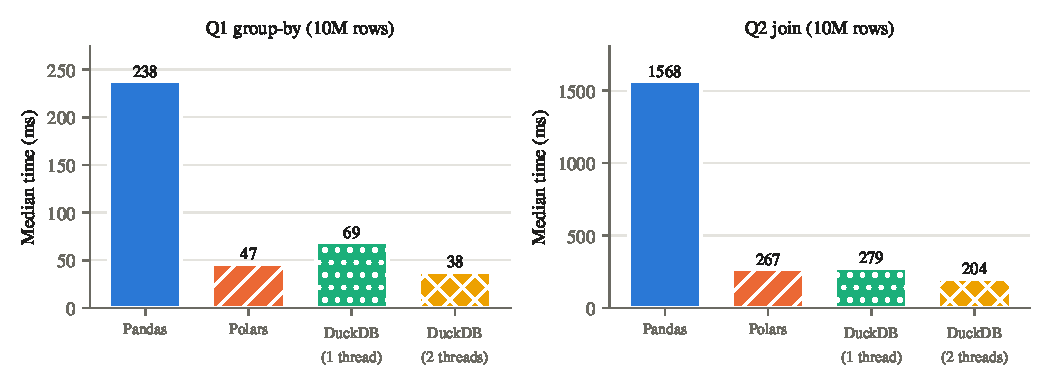
\includegraphics[width=0.9\textwidth]{figures/fig1_query_time.pdf}
\caption{Median query time at 10 million rows for Q1 (group-by) and Q2 (join). Lower is better.}
\label{fig:time}
\end{figure*}

\begin{figure*}[t]
\centering
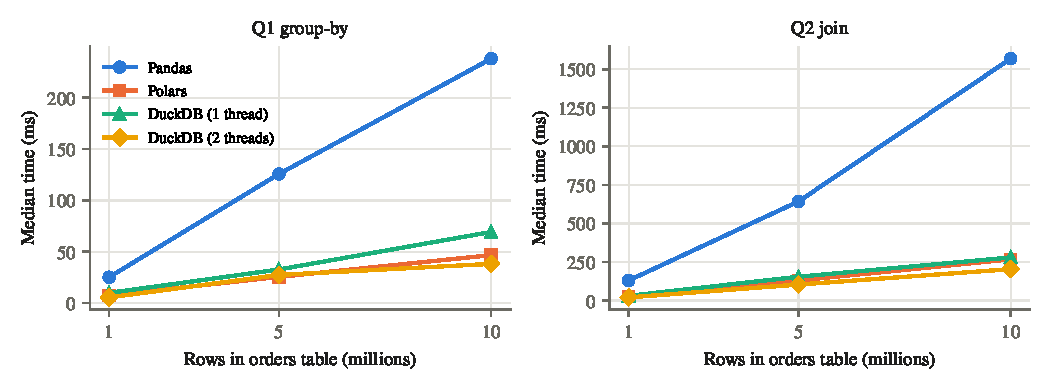
\includegraphics[width=0.9\textwidth]{figures/fig2_scaling.pdf}
\caption{Median query time as the \texttt{orders} table grows from 1 to 10 million rows.}
\label{fig:scaling}
\end{figure*}

\begin{figure}[t]
\centering
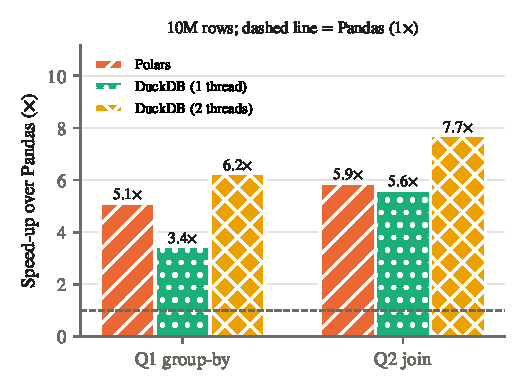
\includegraphics[width=\columnwidth]{figures/fig3_speedup.pdf}
\caption{Speed-up over Pandas at 10 million rows. The dashed line marks Pandas (1$\times$).}
\label{fig:speedup}
\end{figure}

\subsection{RQ1: How Vectorised and GPU Engines Execute Queries}
Pandas evaluates a query step by step: \texttt{merge} produces a complete joined DataFrame, and \texttt{groupby} then scans it again. Its kernels are compiled, but each step reads and writes whole columns in memory and runs essentially on one core~\cite{mozzillo25}. DuckDB instead builds a pipeline in which 2048-value vectors flow from the scan through the hash-join probe straight into the hash aggregate, reading only the needed columns and never materialising the joined table~\cite{raasveldt19,boncz05}. Polars behaves similarly: its lazy plan prunes unused columns, and it runs on Arrow arrays with several threads. Our data show the effect of this design directly. With the \emph{same} single core as Pandas, DuckDB is 3.4$\times$ faster on Q1 and 5.6$\times$ faster on Q2 (Table~\ref{tab:results}). The advantage is larger for the join because Pandas copies all five order columns into the joined result, while DuckDB streams only the two it needs. GPU engines follow the same columnar, data-parallel model with thousands of threads, and their advantage over well-optimised CPU code is bounded mainly by memory bandwidth~\cite{shanbhag20,paul21}. We could not measure a GPU on our machine, so this part of RQ1 rests on the literature.

\subsection{RQ2: Role of SIMD, Columnar Formats and Arrow}
Three hardware-friendly ingredients explain the single-thread gap. \emph{Columnar layout} means that Q1 reads only \texttt{store\_id}, \texttt{amount} and \texttt{quantity}, which are contiguous arrays, instead of whole rows. \emph{Vectorised loops} over these arrays keep data in the CPU cache and let the compiler emit SIMD instructions (AVX2/AVX-512 here) that process several values per instruction~\cite{polychroniou15,kersten18}. \emph{Arrow} provides a shared in-memory columnar standard, so Polars operates directly on Arrow buffers and data moves between tools without conversion~\cite{arrow,lamb24}. Fig.~\ref{fig:scaling} supports this explanation. From 1M to 10M rows, Pandas' Q2 time grows 12.1$\times$, faster than the data, while two-thread DuckDB grows 10.0$\times$, in proportion to the data. Polars' Q1 speed-up rises from 3.4$\times$ to 5.1$\times$. Larger inputs therefore favour the vectorised engines, because fixed per-query costs are amortised and the Pandas join must materialise more intermediate data. We note that our experiment shows the combined effect of these ingredients; it does not isolate SIMD alone.

\subsection{RQ3: Speed-Up and Where It Comes From}
At 10 million rows, the overall speed-up of DuckDB over Pandas is 6.2$\times$ for Q1 and 7.7$\times$ for Q2 (Fig.~\ref{fig:speedup}). Splitting this as described in Section~\ref{sec:method}:
\begin{itemize}
\item Q1: $6.25 = 3.44$ (execution model) $\times\ 1.82$ (threads);
\item Q2: $7.71 = 5.61$ (execution model) $\times\ 1.37$ (threads).
\end{itemize}
The execution-model factor is the larger one in both cases. Moving from one to two threads gives a near-linear 1.82$\times$ for the group-by, whose 100 small per-thread hash tables merge cheaply. The join gains only 1.37$\times$, likely because building the shared hash table on one million customers is partly sequential and probing it is limited by memory bandwidth. Polars, which also uses both cores, lands between the two DuckDB settings (5.1$\times$ and 5.9$\times$). These results agree with Mozzillo et al.~\cite{mozzillo25}, who find Polars much faster than Pandas when data fits in memory, and add the missing explanation: on commodity hardware, most of the gain comes from \emph{how} the query is executed, not from \emph{how many} cores execute it.

\subsection{Threats to Validity}
\emph{Hardware:} the shared cloud VM has only two virtual CPUs and no GPU, so the parallelism factor is a lower bound, and cuDF could not be tested. On a laptop with 8 cores, the thread gain would be larger. Run-to-run noise is visible at 5M rows, where Q1's thread gain is only 1.19$\times$; we reduce noise with a warm-up and the median of ten runs, and record min/max values. \emph{Data:} keys are uniformly distributed, whereas real data are often skewed, which affects hash tables. \emph{Scope:} we time in-memory execution only, so file loading and larger-than-memory behaviour~\cite{kuiper24,kuiper25} are excluded. \emph{Versions:} results depend on library versions, which we pin and report. \emph{Attribution:} the one-thread comparison mixes several effects (vectorisation, SIMD, pipelining, column pruning) that we do not separate further.

%======================================================================
\section{Conclusion and Future Work}\label{sec:conclusion}
We reviewed 18 studies on hardware-conscious query processing and measured Pandas, Polars and DuckDB on group-by and join queries over up to 10 million rows. All engines agreed on every result. At 10M rows, DuckDB was 6.2$\times$ (group-by) and 7.7$\times$ (join) faster than Pandas, and Polars 5.1$\times$ and 5.9$\times$. Running DuckDB on a single thread still gave 3.4$\times$ and 5.6$\times$, so the execution model, not parallelism, accounts for most of the improvement on commodity hardware. The main limitations are the two-core machine, the absence of a GPU and the uniform synthetic data. Future work includes (1)~adding cuDF on a GPU (e.g., a free Colab instance) to measure the GPU factor directly, (2)~running on 8--16-core machines and with skewed or TPC-H data, and (3)~including Parquet scan time to capture the effect of columnar storage end to end.

\section*{Contribution Statement}
\textbf{Krish (S1):} Conceptualisation, project administration, writing -- original draft (Abstract, Introduction, Conclusion), final formatting. \textbf{Krish Singhal (S2):} Investigation (literature search), data curation (literature matrix), writing -- Related Work, citation checks. \textbf{Laksh Kapoor (S3):} Software, methodology, validation (benchmark code, GitHub repository, README), writing -- Methodology and Setup. \textbf{Lucky (S4):} Formal analysis, visualisation, writing -- Results and Discussion, plagiarism check and presentation slides.

\section*{AI Usage Note}
An AI assistant (Claude, Anthropic) was used to help draft text, benchmark code and figures, and to check references. The authors ran all experiments, verified every reference against its source, and reviewed and take full responsibility for all content.

\section*{Code and Data Availability}
Code, data generator, raw results and figures: \url{https://github.com/LakshK001/g14-hardware-accelerated-query}.

\begin{thebibliography}{99}

\bibitem{mckinney10}
W. McKinney, ``Data structures for statistical computing in Python,'' in \emph{Proc. 9th Python in Science Conf. (SciPy)}, 2010, pp. 56--61.

\bibitem{raasveldt19}
M. Raasveldt and H. M\"uhleisen, ``DuckDB: An embeddable analytical database,'' in \emph{Proc. ACM SIGMOD Int. Conf. Manage. Data}, 2019, pp. 1981--1984, doi: 10.1145/3299869.3320212.

\bibitem{polars}
Polars Developers, ``Polars,'' ver. 2.1.0, 2026. [Online]. Available: https://pola.rs

\bibitem{arrow}
Apache Software Foundation, ``Apache Arrow,'' 2026. [Online]. Available: https://arrow.apache.org

\bibitem{boncz05}
P. Boncz, M. Zukowski, and N. Nes, ``MonetDB/X100: Hyper-pipelining query execution,'' in \emph{Proc. Conf. Innovative Data Syst. Res. (CIDR)}, 2005, pp. 225--237.

\bibitem{polychroniou15}
O. Polychroniou, A. Raghavan, and K. A. Ross, ``Rethinking SIMD vectorization for in-memory databases,'' in \emph{Proc. ACM SIGMOD Int. Conf. Manage. Data}, 2015, pp. 1493--1508, doi: 10.1145/2723372.2747645.

\bibitem{zeng23}
X. Zeng, Y. Hui, J. Shen, A. Pavlo, W. McKinney, and H. Zhang, ``An empirical evaluation of columnar storage formats,'' \emph{Proc. VLDB Endow.}, vol. 17, no. 2, pp. 148--161, 2023, doi: 10.14778/3626292.3626298.

\bibitem{shanbhag20}
A. Shanbhag, S. Madden, and X. Yu, ``A study of the fundamental performance characteristics of GPUs and CPUs for database analytics,'' in \emph{Proc. ACM SIGMOD Int. Conf. Manage. Data}, 2020, pp. 1617--1632, doi: 10.1145/3318464.3380595.

\bibitem{paul21}
J. Paul, S. Lu, and B. He, ``Database systems on GPUs,'' \emph{Found. Trends Databases}, vol. 11, no. 1, pp. 1--108, 2021, doi: 10.1561/1900000076.

\bibitem{graefe94}
G. Graefe, ``Volcano---An extensible and parallel query evaluation system,'' \emph{IEEE Trans. Knowl. Data Eng.}, vol. 6, no. 1, pp. 120--135, 1994.

\bibitem{kersten18}
T. Kersten, V. Leis, A. Kemper, T. Neumann, A. Pavlo, and P. Boncz, ``Everything you always wanted to know about compiled and vectorized queries but were afraid to ask,'' \emph{Proc. VLDB Endow.}, vol. 11, no. 13, pp. 2209--2222, 2018, doi: 10.14778/3275366.3275370.

\bibitem{lamb24}
A. Lamb \emph{et al.}, ``Apache Arrow DataFusion: A fast, embeddable, modular analytic query engine,'' in \emph{Companion Proc. ACM SIGMOD Int. Conf. Manage. Data}, 2024, doi: 10.1145/3626246.3653368.

\bibitem{rosenfeld23}
V. Rosenfeld, S. Bre\ss, and V. Markl, ``Query processing on heterogeneous CPU/GPU systems,'' \emph{ACM Comput. Surv.}, vol. 55, no. 2, 2023, doi: 10.1145/3485126.

\bibitem{behm22}
A. Behm \emph{et al.}, ``Photon: A fast query engine for lakehouse systems,'' in \emph{Proc. ACM SIGMOD Int. Conf. Manage. Data}, 2022, doi: 10.1145/3514221.3526054.

\bibitem{pedreira22}
P. Pedreira \emph{et al.}, ``Velox: Meta's unified execution engine,'' \emph{Proc. VLDB Endow.}, vol. 15, no. 12, pp. 3372--3384, 2022, doi: 10.14778/3554821.3554829.

\bibitem{kuiper24}
L. Kuiper, P. Boncz, and H. M\"uhleisen, ``Robust external hash aggregation in the solid state age,'' in \emph{Proc. IEEE 40th Int. Conf. Data Eng. (ICDE)}, 2024.

\bibitem{kuiper25}
L. Kuiper, P. Gro\ss, P. Boncz, and H. M\"uhleisen, ``Saving private hash join,'' \emph{Proc. VLDB Endow.}, vol. 18, no. 8, pp. 2748--2760, 2025, doi: 10.14778/3742728.3742762.

\bibitem{yogatama22}
B. W. Yogatama, W. Gong, and X. Yu, ``Orchestrating data placement and query execution in heterogeneous CPU-GPU DBMS,'' \emph{Proc. VLDB Endow.}, vol. 15, no. 11, pp. 2491--2503, 2022, doi: 10.14778/3551793.3551809.

\bibitem{cao23}
J. Cao, R. Sen, M. Interlandi, J. Arulraj, and H. Kim, ``GPU database systems characterization and optimization,'' \emph{Proc. VLDB Endow.}, vol. 17, no. 3, pp. 441--454, 2023, doi: 10.14778/3632093.3632107.

\bibitem{daase21}
B. Daase, L. J. Bollmeier, L. Benson, and T. Rabl, ``Maximizing persistent memory bandwidth utilization for OLAP workloads,'' in \emph{Proc. ACM SIGMOD Int. Conf. Manage. Data}, 2021, pp. 339--351, doi: 10.1145/3448016.3457292.

\bibitem{liu23}
C. Liu, A. Pavlenko, M. Interlandi, and B. Haynes, ``A deep dive into common open formats for analytical DBMSs,'' \emph{Proc. VLDB Endow.}, vol. 16, no. 11, pp. 3044--3056, 2023, doi: 10.14778/3611479.3611507.

\bibitem{mozzillo25}
A. Mozzillo, L. Zecchini, L. Gagliardelli, A. Aslam, S. Bergamaschi, and G. Simonini, ``Evaluation of dataframe libraries for data preparation on a single machine,'' in \emph{Proc. 28th Int. Conf. Extending Database Technol. (EDBT)}, 2025. [Online]. Available: https://arxiv.org/abs/2312.11122

\bibitem{harris20}
C. R. Harris \emph{et al.}, ``Array programming with NumPy,'' \emph{Nature}, vol. 585, no. 7825, pp. 357--362, 2020, doi: 10.1038/s41586-020-2649-2.

\bibitem{hunter07}
J. D. Hunter, ``Matplotlib: A 2D graphics environment,'' \emph{Comput. Sci. Eng.}, vol. 9, no. 3, pp. 90--95, 2007, doi: 10.1109/MCSE.2007.55.

\end{thebibliography}

\end{document}
